\chapter{Efficient solution of the linear systems}
\chaptermark{Solution of linear systems}
\label{sec:solution-strategies}

When we apply implicit time integration schemes, a FEM spatial discretisation and the Newton-Raphson method for linearisation (as discussed in \cref{sec:time-discretisation,sec:galerk-meth-llg}) to the LLG equation we are left with the problem of solving a sequence of large sparse linear systems to obtain the approximate solution.
With the addition of FEM/BEM for calculation of magnetostatic fields (as discussed in \cref{sec:hybr-finit-elem}), the linear systems to be solved become larger and more complex.
In this \thisref{sec:solution-strategies} we discuss solution strategies for these systems.

In \cref{sec:llg-only-system} we first discuss the solution of the systems required in the calculation of the magnetostatic field assuming the magnetisation is known.
We then discuss methods of solving the linear systems for the LLG equation assuming the magnetostatic field is known.
This is non-trivial because of the inclusion of the dense BEM matrix.

In \cref{sec:solut-coupl-syst} we describe two efficient methods for the solution of the LLG equation with magnetostatics: a ``monolithic'' (\ie fully coupled) approach and a semi-implicit approach.
The semi-implicit approach breaks the problem into a sequence of easily solved linear systems but at the cost of modifying the time integration scheme.
The monolithic approach uses efficient numerical methods to solve the full linear system and preserves all properties of the time integration scheme, such as stability and geometric integration properties.
In particular the energy conservation property of IMR requires the use of a monolithic approach (see \cref{sec:proof-energy-prop}).
Except for the simplest preconditioner, \cref{eq:90}, the preconditioners for the monolithic approach are novel.

Finally, in \cref{sec:numer-exper-fem-bem-systems}, we present some numerical experiments demonstrating the effectiveness of the proposed linear solvers for the systems resulting from both the semi-implicit and monolithic approaches.



\section{Solution of decoupled systems}
\label{sec:llg-only-system}

In \thisref{sec:llg-only-system} we consider the solution of the magnetostatic and LLG problems in isolation (\ie the LLG problem is solved assuming that the magnetostatic field is a known function and vice-versa).
Such methods are important building blocks for the solution of the coupled system.

Firstly we consider the two linear systems solved in the magnetostatic field calculations: these are both Poisson systems (see \cref{eq:phi-bem-continuous} and \cref{eq:poisson-jacobian}), which are well studied.
One efficent and robust method for solving Poisson systems on unstructured grids is to use the method of conjugate gradients (CG) with algebraic multigrid (AMG) as a preconditioner \cite{Henson2002}.

Note that the Poisson blocks $\Am$ do not depend on $\phim$, $\phione$ or $\mv$ (\ie the Poisson problems are linear).
This means that when solving these parts of the problem the Newton-Raphson iteration is not required (or if used it will converge in a single iteration assuming that the linear solve is sufficiently accurate).
Also the $\Am$ matrices only depend on the geometry and so can be computed once and stored for reuse throughout the duration of the simulation (and similarly for the coarsening information required by the AMG preconditioner).


Now we focus on the sequence of linear systems resulting from solving the LLG equation with the Newton-Raphson method, \cref{eq:llg-jacobian}.
There do not appear to be any solvers which are efficient, robust and scale optimally with matrix size in the literature.
We try two solvers in our implementation, unfortunately neither are expected to be efficient for large matrix sizes and large time steps.

The first method used is a direct solve by LU decomposition.
As discussed in \cref{sec:direct-methods} this method is extremely robust but is very slow for large matrices, particularly for problems in three spatial dimensions.

The second method is to use a Krylov solver preconditioned by an incomplete LU decomposition (ILU), inspired by \cite{Suess2002}.
This method is expected to be efficient for medium sized problems and/or small time steps, especially in 2D or thin film problems where the FEM nodes are less coupled.
However the effectiveness is strongly dependent on the diagonal dominance of the matrix.
In particular as the volume of the elements decreases or the time step size increases the matrix will become less diagonally dominant and the effectiveness will decrease.
Hence this method is not expected to scale optimally to fine meshes or to be robust with respect to varying parameters.

% Unfortunately we have not had time to research more effective solvers for the LLG system.
% maybe write something abount what these might be? block based AMG smoothers (as used for fixed point)? block preconditioners with AMG underlying? [Milan/Matthias: what's the big difference?]

\section{Solution of the coupled LLG-magnetostatics system}
\label{sec:solut-coupl-syst}

We now consider the solution of the combined LLG and FEM/BEM magnetostatics system.
Unlike typical FEM computations, these linear systems are not entirely sparse: the BEM matrix, $\bm$, (derived in \cref{sec:discretisation}, \cref{eq:17}) appears as a dense block in the Jacobian.
In this \thisref{sec:solut-coupl-syst} we describe two approaches to efficiently solve the resulting non-linear system despite this issue.

In \cref{sec:semi-implicit-bem} we describe the first approach which involves replacing our implicit time integration scheme with an ad-hoc semi-implicit version which handles the magnetostatic calculation explicitly.
This means that only decoupled solves for $\phione$, $\phi$ and $\mv$ are required at each time step, and the dense block, $\bm$, only appears as a matrix-vector multiply.
However it also means that we are no longer using the time integration methods discussed in \cref{sec:some-implicit-time-integrators}, instead we are using some new scheme.

The second approach, described in \cref{sec:fully-implicit-bem}, is to construct a linear solver which can efficiently handle the dense block.
We present a novel solver which consists of a Krylov solver combined with a preconditioner and an efficient representation of the BEM block.
This approach has the benefit that all of the properties of the original time integration schemes carry over to the coupled problem.
In particular when using this approach the IMR retains the energy property described in \cref{sec:proof-energy-prop}, which is the most interesting of its geometrical integration properties.\footnote{A number of integration schemes can obtain length conservation: Cayley transform methods \cite{Lewis2003}, semi-analytical methods \cite{Wiele2010} and various types of semi-implicit midpoint rule methods \cite{Spargo2003} \cite{Mentink2010} (including the one described in \cref{sec:semi-implicit-bem}).}
Additionally it may be useful for stochastic problems (\ie when thermal fields are involved, see \cref{sec:temperature-effects}), since in this case only a few time integration schemes are known to converge to the correct solution.
The implicit midpoint rule is one of these schemes, but the semi-implicit modification is likely to remove this property \cite{DAquino2006}.

Before describing these approaches in more detail, we briefly discuss the implementation of the monolithic coupling between the LLG and magnetostatic problems, and the structure of the resulting Jacobian.

\subsection{Residuals and Jacobian for the monolithically coupled system}
\label{sec:bem-jacobian-structure}

As mentioned in \cref{sec:discretisation} the pair of potentials used in the FEM/BEM method is similar to that of the simplified magnetostatic potential discussed in \cref{sec:galerk-meth-llg}.
There are two differences: the first is that there is no coupling from the auxiliary potential $\phione$ to the LLG equation, and hence no corresponding block in the full Jacobian.

The second difference is that there is an additional coupling between the boundary values of $\phione$ and the boundary values of $\phim$.
This coupling between the BEM part (a collocation method) and the FEM part (a Galerkin method) is implemented using the following residual vector:
\newcommand{\rphimb}{\rphi_\boundd}
\begin{equation}
  \rphimb(\phimdis_\boundd, \phionedis_\boundd) = \bm \phionedis_\boundd - \phimdis_\boundd,
  \label{eq:89}
\end{equation}
where $\mydiscrete{x}_\boundd$ denotes the vector of values of $x$ at the boundary nodes.
This residual is included as normal in the non-linear solve and simply enforces the condition $\phimdis_\boundd = \bm \phionedis_\boundd$ from \cref{eq:10}.
Note that we cannot enforce the condition in the standard way (by pinning the values at the boundary nodes to the appropriate values) because the condition is obtained as part of the solve.

A natural consequence of \cref{eq:89} is that the BEM matrix is a block of the Jacobian:
\begin{equation}
  \pd{\rphimb}{\phionedis_\boundd} = \bm,
  \label{eq:92}
\end{equation}
where we have again used the notation that $\pd{\av}{\bv}$ is the Jacobian of the derivatives of $\av$ with respect to $\bv$, as in \cref{eq:jac-def}.
Also note that the diagonal Jacobian block for the boundary values of $\phim$ is simply the identity matrix
\begin{equation}
  \pd{\rphimb}{\phimdis_\boundd} = -\Idm.
  \label{eq:91}
\end{equation}

\newcommand{\Amm}{\Am_\phim}
\newcommand{\Amu}{\Am_\phione}
\newcommand{\zm}{0}
\newcommand{\Abound}{\Am_{\phim\boundd}}

\newcommand{\scalemath}[2]{\scalebox{#1}{\begin{math} {#2} \end{math}}}

\newcommand{\Aprime}{\scalemath{0.5}{\begin{matrix} \Amm     & \Abound \\ \zm      & -\Idm \end{matrix}}}
\newcommand{\Gprime}{\scalemath{0.5}{\begin{matrix} \zm  & \zm \\ \zm  & \bm \end{matrix}}}
\newcommand{\Qprime}{\scalemath{0.5}{\begin{matrix} \Qm \\ \zm \end{matrix}}}


Combining the above with the Jacobian matrix as derived in \cref{sec:llg-magn-coupl}, the complete Jacobian is
\begin{equation}
  \Jm =
  \scalemath{2}{
    \begin{pmatrix}
      \Fm        & \Pm     &  \zm \\
      \Qprime &   \Aprime &  \Gprime  \\
      \Qm       &  \zm       &   \Amu
    \end{pmatrix}
  },
  \label{eq:16}
\end{equation}
where $\Abound = \pd{\phimh}{\phimdis_\boundd}$ is the Jacobian of the bulk $\phim$ values with respect to the boundary values.
The order of blocks is $\mv$, $\phim$, $\phione$.
The blocks corresponding to derivatives of the $\phim$ residual are broken into sub-blocks for the bulk and boundary values due to the BEM coupling.
The overall Jacobian is a square matrix with number of rows $\nrow = 5\Nn$, where $\Nn$ is the number of nodes.
The LLG block, $\Fm$, is of size $3\Nn\times 3\Nn$, the Poisson block, $\Amu$, is of size $\Nn \times \Nn$.
The smaller Poisson block, $\Amm$, is of size $\Nbul \times \Nbul$, where $\Nbul$ is the number of bulk nodes.
The identity and BEM matrices are of size $\Nb \times \Nb$, where $\Nb$ is the number of boundary nodes.

For brevity we write the Jacobian, \cref{eq:16}, as
\begin{equation}
  \Jm =
  \begin{pmatrix}
    \Fm       & \Pm     &  \zm \\
    \Qm' &   \Amm' &  \Gm'  \\
    \Qm       &  \zm       &   \Amu
  \end{pmatrix}.
\end{equation}


It is worth noting that a slightly different Jacobian struture could be obtained by modifying the derivation in \cref{sec:appl-magn-calc}.
Instead of using $\phim = \phione + \phitwo$ to eliminate $\phitwo$, we could use $\hms = - \grad ( \phione + \phitwo)$ and eliminate $\phim$.
This would result in both of the potentials having a $\Pm$ block, but only one of them having a $\Qm$ block.
It would also reduce the diagonal dominance of $\bm$.
We have not experimented with this alternative formulation.

The linear system to be solved at each Newton step is (see \cref{sec:newt-raph})
\begin{equation}
  \jac \corr = -\resi,
  \label{eq:87}
\end{equation}
where $\resi$ is the vector of the current discrete Newton residuals for $\mv$, $\phim$ and $\phione$; and we need to find the Newton update $\corr = [\corr\mvdis, \corr\phimdis, \corr\phionedis]^T$.


\subsection{The semi-implicit approach}
\label{sec:semi-implicit-bem}

One approach, which avoids solving the complete non-linear system, is to break the monolithic system into multiple coupled but simpler problems.
This can be achieved by using implicit calculations for the LLG parts as normal, but treating the magnetostatic calculations explicitly.
The resulting scheme then only requires independent calculations of the magnetostatic field and the magnetisation as described in \cref{sec:llg-only-system}.
Since the magnetostatic fields are typically much weaker than the exchange field we hope that the stability of the scheme will not be greatly reduced.

An outline of the algorithm to compute the step from time $t_n$ to $t_{n+1}$ is as follows:
\begin{algorithm}[H]
  Extrapolate the magnetostatic potential (using $\phim_n$, $\phim_{n-1}$) to time $t_{n+1}$, call the result $\hat{\phim}_{n+1}$\;
  Use $\hat{\phim}_{n+1}$ to calculate $\mv_{n+1}$ using an implicit time integration scheme (a non-linear solve of the $\Fm$ block)\;
  Calculate $\phione_{n+1}$ using $\mv_{n+1}$ (a Poisson solve)\;
  Use boundary values of $\phione_{n+1}$ to calculate the boundary values of $\phim_{n+1}$ (a matrix-vector multiply with the BEM matrix)\;
  Calculate $\phim_{n+1}$ everywhere using these Dirichlet boundary conditions and $\mv_{n+1}$ (a Poisson solve)\;
\end{algorithm}

Note that we use an extrapolation of the magnetostatic potential, $\phim$, to $t_{n+1}$ rather than computing it using a step of an explicit time integration scheme because there is no time derivative in the equations for $\phim$.
A similar method without the extrapolation step been used previously, see \eg \cite{Schrefl1997}.

% Alternatively we could take an explicit step of the LLG and use the result to calculate $\hat{\phim}_{n+1}$.
% Inside an adaptive time integration scheme the explicit step used to estimate the local truncation error could be reused for this purpose.
% We have not experimented with this idea.

For step 1 of the algorithm we require a second order accurate extrapolation in order to ensure that the local truncation error of the overall time integration scheme remains second order.
A simple second order extrapolation formula (based on Lagrange interpolation \cite[312]{Kincaid2002}) is
\begin{equation}
  \label{eq:65}
  f(t_{n+1}) = \frac{t_{n+1} - t_n}{t_{n-1} - t_n}f(t_{n-1}) + \frac{t_{n+1} - t_{n-1}}{t_n - t_{n-1}}f(t_n),
\end{equation}
replacing differences in time with the appropriate time steps gives:
\begin{equation}
  \label{eq:66}
  \hat{\phim}_{n+1} = \frac{-\dtx{n+1}}{\dtn} \phim_{n-1} + \frac{\dtx{n+1} + \dtn}{\dtn} \phim_n.
\end{equation}
Note that if we are using the implicit midpoint rule we need to extrapolate $\phim$ to the midpoint rather than $t_{n+1}$, hence we use $\dtx{n+1} = \dtx{n+1} /2$ in the above equation.

%  write out LTE for this scheme somehow?

Unfortunately this method requires two initial values for the magnetostatic potential values.
The additional value can be generated by directly calculating the potential if the magnetisation values at two initial times are known.
Otherwise the first can be calculated from the initial condition and the potential at a second time can be calculated by taking one step of a monolithic method or a (much smaller) time step using a first order extrapolation formula.

The linear and non-linear systems resulting from the application of this algorithm are exactly those discussed in \cref{sec:llg-only-system}.


% could mention semi-implicit + fixed point iteration approach? No one's ever used it in micromagnetics as far as I know.


\subsection{The monolithic approach}
\label{sec:fully-implicit-bem}

The alternative to the semi-implicit approach described above is to find an efficient way to solve the full system \cref{eq:16,eq:87}, this is referred to as a fully coupled or monolithic approach.
The major difficulty is that the system contains a dense block, meaning that any operations (\eg LU decomposition, multiplication) on J will be significantly slower than for a sparse Jacobian.
We use a combination of techniques to reduce this negative effect of the BEM block.

The first and most important technique is the use of a Krylov solver, this has two benefits.
Firstly, as mentioned in \cref{sec:krylov-solvers}, a Krylov solver (with an effective preconditioner) is typically significantly faster and more memory efficient than a direct solver.
Secondly, using a Krylov solver rather than a direct solve or a multigrid-based solver means that all that is required of $\jac$ is the computation of matrix-vector products.
This allows us to split $\jac$ into separate matrices as
\begin{equation}
  \begin{aligned}
    \jac &=
    \begin{pmatrix}
      \Fm       & \Pm     &  \zm \\
      \Qm' &   \Amm' &  \zm  \\
      \Qm       &  \zm       &   \Amu
    \end{pmatrix}
    +
    \begin{pmatrix}
      \zm       & \zm     &  \zm \\
      \zm       &  \zm    &  \Gm'  \\
      \zm       &  \zm    &  \zm
    \end{pmatrix},
    \\
    &= \jac_S + \jac_D.
  \end{aligned}
\end{equation}
The matrix-vector product can be computed as
\begin{equation}
  \jac \xv = \jac_S \xv + \jac_D \xv,
\end{equation}
\ie the dense and sparse parts can be stored and used completely independently.

This leads us to the second component of our method: the use of a hierarchical matrix format for the BEM block \cite{Borm2003,Forster2003,Knittel2011}.
This format uses techniques similar to the fast multipole method to use computationally cheap (in both time and memory) but less accurate approximations to the matrix where possible, without compromising overall accuracy.
It reduces the computational cost for a matrix-vector product with the dense block to $\order{\Nb \log \Nb}$.
Since the number of boundary nodes $\Nb$ is typically less than the total number of nodes in the problem this can allow the cost of matrix-vector products of $\jac$ to be optimal (\ie $\order{\nrow}$) depending on the geometry.
It also reduces the memory requirements for the block to $\order{\Nb \log \Nb}$.
This introduces a small additional error, but it has been shown that the size of the error can be made significantly less than the FEM approximation error by choosing appropriate parameters \cite[77]{Knittel2011}.
The use of such formats has recently become fairly common in the application of the hybrid FEM/BEM method to micromagnetics problems.

The third and final component in our efficient solver is a cheap and effective preconditioner for the linear system.
Some approaches to constructing such a preconditioner will be discussed in the following section.


\subsubsection{Preconditioning strategies}
\label{sec:bem-solver-strategies}


In this section we give a number preconditioning approaches for the monolithic system with the Jacobian \cref{eq:16}.
The aim is to construct a preconditioner which gives an approximately constant number of Krylov solver iterations independently of all problem and discretisation parameters but which is also quick to set up and does not consume a large quantity of memory.

The first preconditioner is very simple: we use a direct solve (using LU decomposition) of the sparse part of $\Jm$, \ie
\begin{equation}
  \preca = \jac_S =
  \begin{pmatrix}
    \Fm       & \Pm     &  \\
    \Qm'       & \Amm'    &   \\
    \Qm       &         &   \Amu
  \end{pmatrix}.
\label{eq:90}
\end{equation}
This preconditioner, while much more efficient than a direct solve including the dense block, still suffers from all the usual problems associated with a direct solver (\ie expensive in both memory and computation time when $\Nn$ is large).
However, we are interested in its properties as a test of the effectiveness of dropping the $\Gm'$ block from the preconditioner.

A number of other FEM/BEM based models use an approach similar to preconditioner $\preca$ \cite{Suess2002}, except that the preconditioner is solved by an inner Krylov solver, rather than a direct solve.
This makes the computational cost feasible for realistic problems, but has two issues:
The first is that technically an inner Krylov solve cannot be used as a preconditioner because it does not apply the same operation at each step of the outer solve \cite{Saad1993}.
This issue can be resolved by using an outer Krylov solver known as Flexible GMRES which accounts for this.
The second issue is that a full inner Krylov solve is run at \emph{every iteration} of the outer Krylov solve, which is computationally expensive compared to a standard preconditioner (but still cheaper than a direct solve for sufficiently large problems).
However we are only interested in $\preca$ as a test of the effect of dropping the dense matrix on the iteration counts, hence we do not pursue this further.

Our second and third preconditioners are more ambitious: motivated again by the fact that the magnetostatic field is usually significantly weaker than the exchange effective field we drop an LLG-magnetostatics coupling block in order to make the preconditioner block triangular.
It can then be inverted by inverting only the diagonal blocks (exactly or approximately) and using block back/forward substitution.
The two preconditioners, resulting from dropping different LLG-magnetostatics blocks, are:
\begin{equation}
  \precb =
  \begin{pmatrix}
    \Fm       &           &  \\
    \Qm'       & \Amm'&   \\
    \Qm       &           &   \Amu
  \end{pmatrix},
  \qquad
  \precc =
  \begin{pmatrix}
    \Fm       & \Pm       &  \\
    & \Amm' &   \\
    \Qm       &           &   \Amu
  \end{pmatrix},
  \label{eq:ms-block-prec-drop-p}
\end{equation}
where the blocks in $\precc$ can be reordered to give a block triangular matrix, but we write them in the same order as used elsewhere for consistency.
However, inverting $\precb$ or $\precc$ directly would still require an expensive, in terms of both memory and set up time, direct solve of the three diagonal blocks $\Fm$, $\Amm'$ and $\Amu$.
Ideally we want to approximate these inverses by some cheap iterative process instead.

Based on the fact that AMG is known to be an optimal preconditioner for Krylov solves of Poisson problems, we apply an AMG approximation for the $\Am$ blocks.
Using this approximation we define two semi-inexact preconditioners
\begin{equation}
  \parinexact{\precb} =
  \begin{pmatrix}
    \Fm       &           &  \\
    \Qm'       & \inexact{\Amm'} &   \\
    \Qm       &           &   \inexact{\Amu}
  \end{pmatrix},
  \qquad
  \parinexact{\precc} =
  \begin{pmatrix}
    \Fm       & \Pm       &  \\
    & \inexact{\Amm'} &   \\
    \Qm       &           &  \inexact{\Amu}
  \end{pmatrix},
  \label{eq:ms-block-prec-drop-p}
\end{equation}
where we use $\inexact{x}$ to denote that the block is approximated iteratively and
\begin{equation}
  \inexact{\Amm'} =
  \begin{pmatrix}
    \inexact{\Amm}     & \Abound \\
    \zm      & -\Idm
  \end{pmatrix},
\end{equation}
\ie only the Poisson block of $\Amm'$ is approximated by AMG, the rest can be solved by block back/forward substitution.

As a final fully-inexact (\ie using only cheap approximations with iterative methods) preconditioner we try approximating the $\Fm$ block using ILU.
However we should expect poor performance for large matrix sizes and time steps, similar to the case of pure-LLG solves preconditioned with ILU as discussed in \cref{sec:llg-only-system}.
We define two fully-inexact preconditioners using this approximation in addition to the AMG approximation for the Poisson blocks discussed above:
\begin{equation}
  \inexact{\precb} =
  \begin{pmatrix}
    \inexact{\Fm} &           &  \\
    \Qm'       & \inexact{\Amm'} &   \\
    \Qm       &           &   \inexact{\Amu}
  \end{pmatrix},
  \qquad
  \inexact{\precc} =
  \begin{pmatrix}
   \inexact{\Fm}       & \Pm       &  \\
    & \inexact{\Amm'} &   \\
    \Qm       &           &  \inexact{\Amu}
  \end{pmatrix}.
  \label{eq:ms-block-prec-drop-p}
\end{equation}


\section{Numerical experiments}
\label{sec:numer-exper-fem-bem-systems}

% linear scale for problem size for Milan?
% show full solver times? -- probably not interesting in general, but would be good to show at least one hlib vs dense...

We now test the performance and robustness of the linear solvers described in \thisref{sec:solution-strategies}.
A comparison of the performance and stability of the monolithic and semi-implicit approaches (using the solvers developed here) will be performed in \cref{cha:numer-experiments}.


\subsection{Problem definition and implementation details}

In order to perform these experiments we need a representative example problem.
We do not use the \mumag standard problem \#4 because the hybrid FEM/BEM method for magnetostatic calculations is particularly ill-suited for such thin film problems (as discussed in \cref{sec:bound-elem-meth}).
The performance on the standard problem would be irrelevant for realistic problems using this method and the computational cost would be unnecessarily large.

Since the majority of practical FEM micromagnetics calculations are in three dimensions our test case should also be 3D.
It also must have sharp corners or edges, in order to include any effect of near singular integrals in the FEM/BEM method.
Based on these considerations we choose to test the solvers on an $L\times L \times L$ cube with $L=1$ exchange length.

When testing solvers it is convenient to chose the initial condition such that non-trivial dynamics occur immediately and relevant results can be obtained with only a single time step.
As such the initial magnetisation is chosen to be
\begin{equation}
  \mv_0(x, y, z) = \threevec{\sin(2\pi x/50) + \sin(2\pi y/50)}{\cos(2\pi x/50) + \cos(2 \pi y/50)}{1.0 - m_y - m_z}.
\end{equation}
Note that a wavelength of $50$ was chosen to ensure that even relatively unrefined meshes are able to resolve the initial state.
The problem geometry and initial conditions are illustrated in \cref{fig:cube-initial-condition}.

\begin{figure}
  \centering
  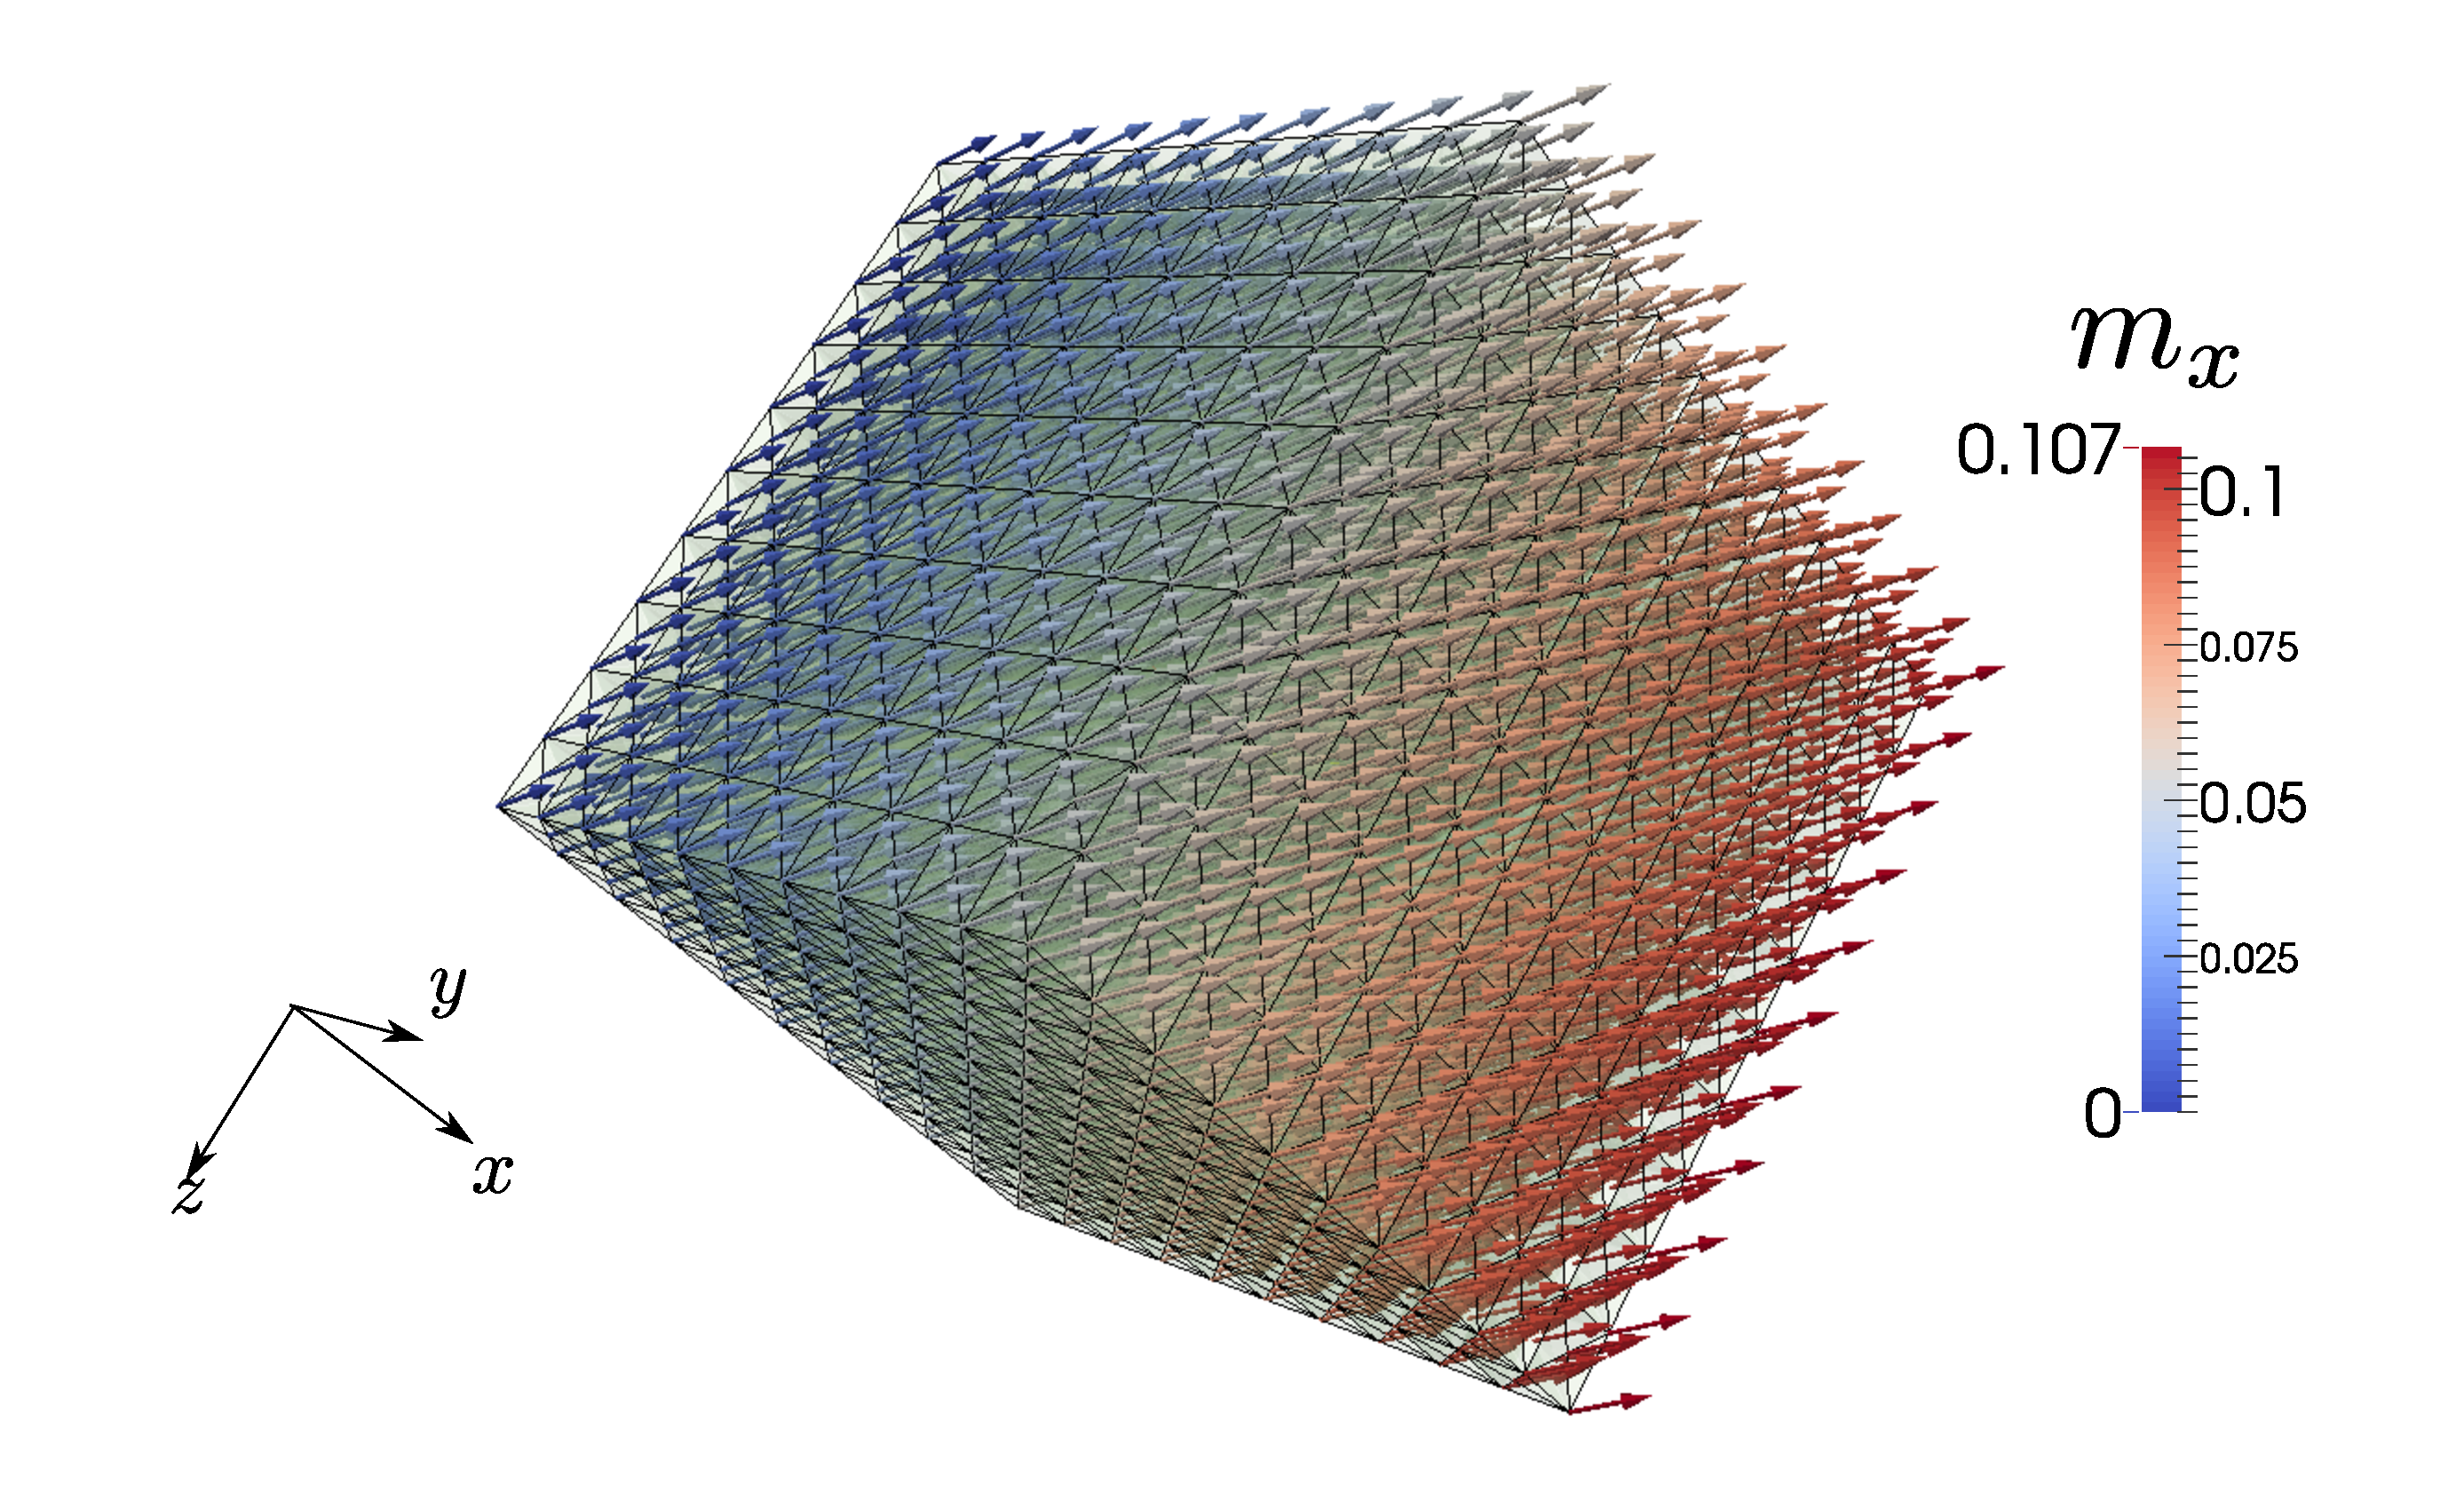
\includegraphics[width=0.8\textwidth]{images/itsacube}
  \caption{The test problem used for the linear solvers in the state at time $t=0$.}
  \label{fig:cube-initial-condition}
\end{figure}


We use a range of damping and anisotropy parameters: $\dampc = 0, 0.01, 1$, $\kone = 0, 0.1$.
 % I should really have done $L=1,10,100$ (equivalent to varying exchange coeff), do it if there's time.
We use zero applied field to avoid inducing accidental symmetries.
Time steps of sizes $\dtn = 0.01, 0.1, 0.5, 1.0$ are chosen, and meshes with $\Nn= 71, 791, 5631, 42461$ nodes (note that the number of rows/columns in the Jacobian is roughly 5 times the number of nodes).
We use both the nodal quadrature discussed in \cref{sec:local-nodal-integr} and a standard Gaussian quadrature.
Since the only effect of changing the time integration methods on the linear systems is a small change to the constant in the time derivative terms we only run experiments using IMR.

The solvers are run both with and without the use of a hierarchical matrix representation for the dense $\Gm$ block.
We use the \hlib library \cite{hlib-website} with patches from \nmag \cite{nmag-website} allowing a collocation BEM approach.
For compatibility with this library we use a tetrahedral mesh.
We use the HCA II algorithm with parameters based on those used by Knittel \cite{Knittel2011}:
$\epsilon_{ACA} = 10^{-5}$,
minimum leaf matrix size $n_{\text{min}}= 30$,
admissibility criterion $\eta = 0.25$,
polynomial interpolation order $p=4$, and
numerical quadrature order $q=3$.
We also use adaptive recompression with $\epsilon = 10^{-3}$.

The CG and GMRES solvers used are \oomph's built-in implementations with relative convergence tolerances of $10^{-8}$.
GMRES with no restarts and left preconditioning is used for to ensure reliable convergence and reliable residual norms.
LU decomposition is implemented using the \superlu package \cite{superlu}.
The AMG implementation used as a preconditioner for Poisson matrices/blocks is \hypre's BoomerAMG \cite{hypre}.
One V(1,1) cycle with Gauss-Seidel smoothing, CLJP coarsening and a connection strength threshold of $0.7$ is used.
The ILU preconditioner used for LLG matrices/blocks is \hypre's Euclid with one level of fill in and no drop tolerance (ILU without fill-in was also tried but was extremely ineffective).


All experiments are run in serial on a desktop computer with an Intel Core i7-3820 processor running at 3.6GHz and 16GB of RAM.


\subsection{Results}

\Cref{fig:its-ilu-decoupled} shows the mean (over a single Newton solve) number of GMRES iterations required to solve the LLG-only system, \cref{eq:llg-jacobian}, using ILU-1 preconditioning (\ie with magnetostatics handled by the semi-implicit approach).
As is expected for a general-purpose preconditioner it is effective for small matrix sizes, but becomes less effective for large problems and as the time step size increases.
% In fact for the largest $\Nn$ with the largest time steps ($\dtn = 1.0$) the solver does not converge with 400 iterations for some parameters.
Note that the plot includes all values of the physical parameters, both quadratures and both $\Gm$ block formats, but these do not appear to have a major impact on the effectiveness of the preconditioner.
The mean preconditioner setup times this preconditioner are shown in \cref{fig:times-ilu-decoupled}.
As with the iteration counts, the setup times become significantly larger as $\Nn$ grows.

\begin{figure}
  \centering
  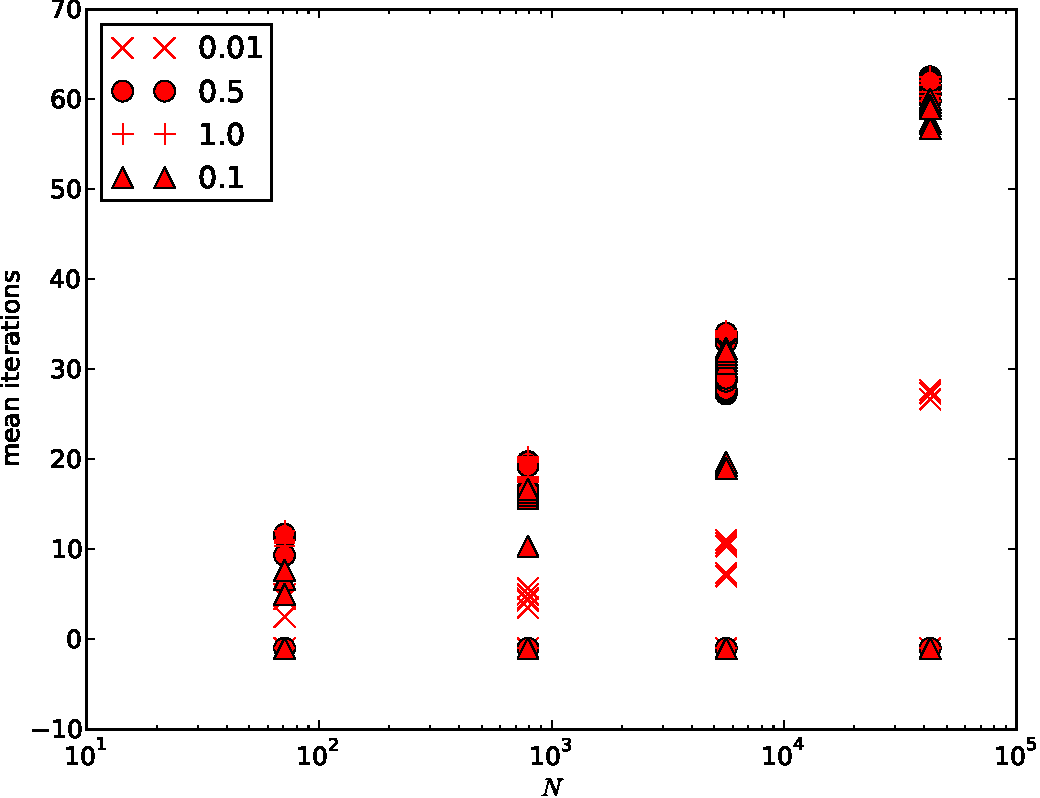
\includegraphics[width=0.8\textwidth]{plots/linear_solvers/ilu-1decoupleddummy-meanofnsolveritersvsinitialnnode.pdf}
  \caption{GMRES iterations to converge against problem size for the decoupled LLG preconditioned by ILU(1). The legend indicates the time step size.}
  \label{fig:its-ilu-decoupled}
\end{figure}

\begin{figure}
  \centering
  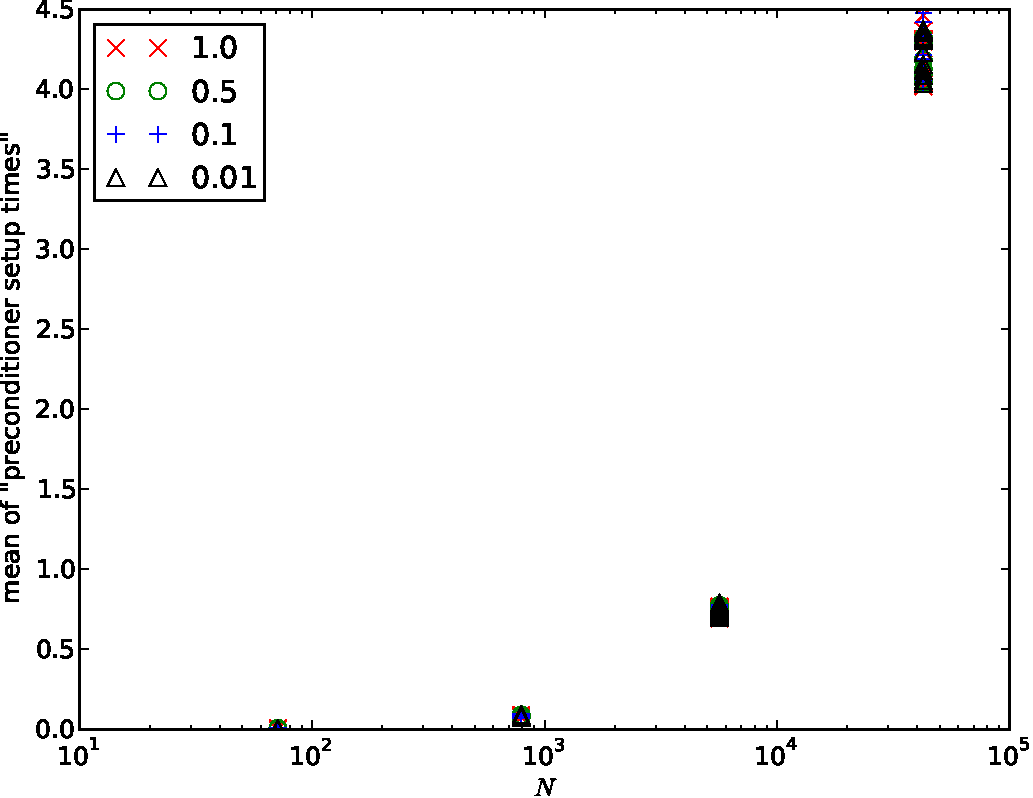
\includegraphics[width=0.8\textwidth]{plots/linear_solvers/ilu-1decoupleddummy-meanofpreconditionersetuptimesvsinitialnnode.pdf}
  \caption{Time in seconds to set up an ILU(1) preconditioner against problem size for the decoupled LLG block. The legend indicates the time step size.}
  \label{fig:times-ilu-decoupled}
\end{figure}


Next we consider the monolithic system \cref{eq:16} solved using preconditioner $\preca$, recall that this uses a direct solve of the sparse part of the Jacobian.
The iteration counts are shown in \cref{fig:its-p1-exact}.
Note that they are roughly independent of the number of nodes and vary only slightly with time step and the various other parameters.
However the preconditioner setup times, shown in \cref{fig:times-p1-exact}, rapidly increase with increasing matrix size as would be expected from a direct solve.
Also, due to the direct solve, the memory usage of this preconditioner is large.
Note that some data for the largest $\Nn$ are missing, this is because the memory required was more than the 16GB available.

\begin{figure}
  \centering
  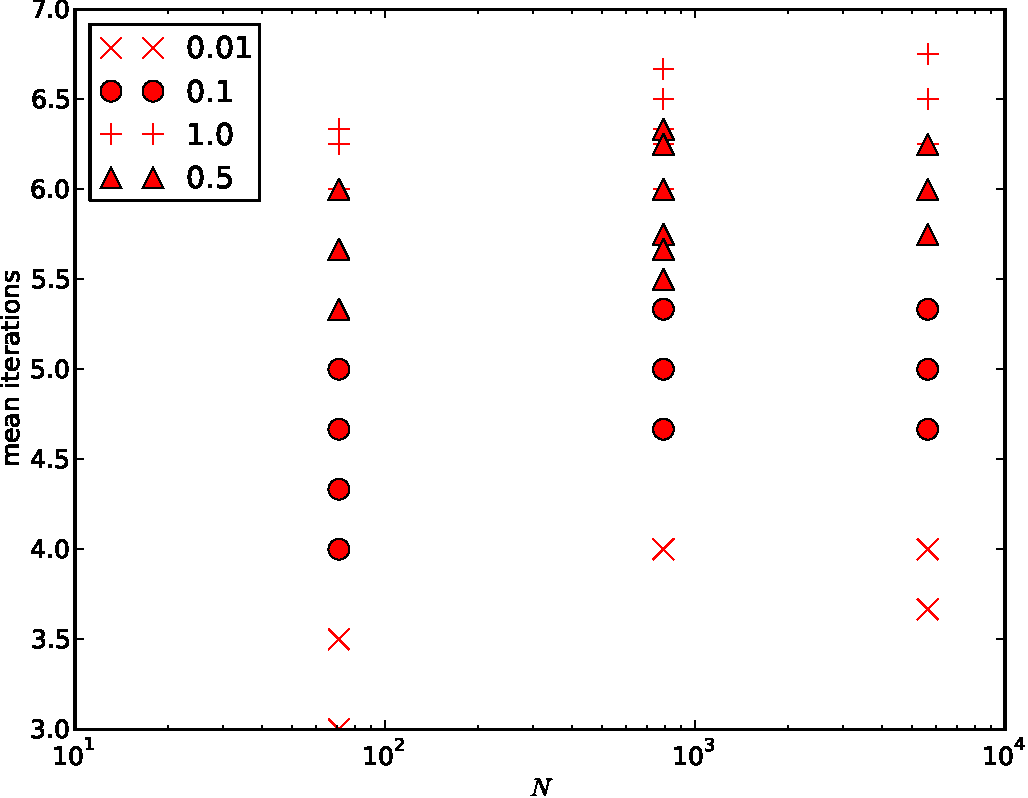
\includegraphics[width=0.8\textwidth]{plots/linear_solvers/som-main-exactimplicitdummy-meanofnsolveritersvsinitialnnode.pdf}
  \caption{GMRES iterations to converge against problem size for the monolithic system preconditioned by $\preca$ (inverted by LU decomposition).
The legend indicates the time step size.
Some data points for the largest $\Nn$ are missing due the LU factors requiring more than 16GB of memory.
}
  \label{fig:its-p1-exact}
\end{figure}


\begin{figure}
  \centering
  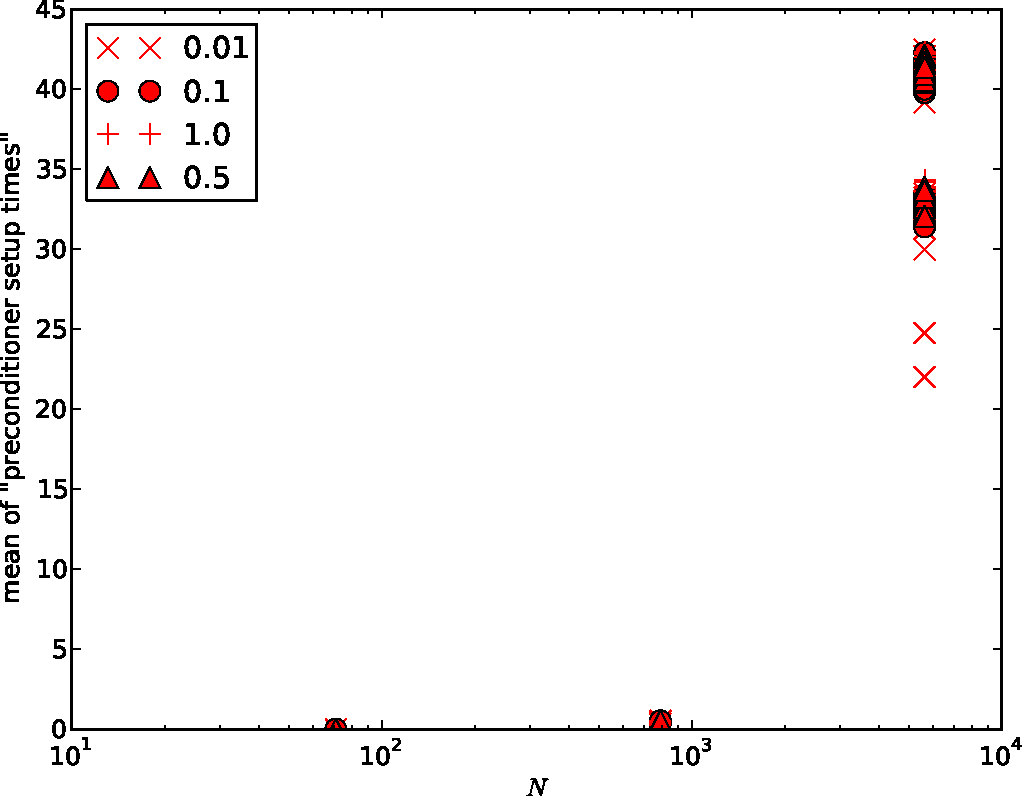
\includegraphics[width=0.8\textwidth]{plots/linear_solvers/som-main-exactimplicitdummy-meanofpreconditionersetuptimesvsinitialnnode.pdf}
  \caption{Time in seconds to set up $\preca$ (inverted by LU decomposition) against problem size for the monolithic system.
    The legend indicates the time step size.
    Some data points for the largest $\Nn$ are missing due the LU factors requiring more than 16GB of memory.
}
  \label{fig:times-p1-exact}
\end{figure}


Now we consider the partially-inexact preconditioners $\parinexact{\precb}$ and $\parinexact{\precc}$, which were designed to reduce the setup time and memory issues of $\preca$ by inverting part of the preconditioner approximately using iterative methods.
The iteration counts are shown in \cref{fig:its-p23-exact}, we see that for both preconditioners the number of iterations increases only slightly as the number of nodes increases and that the various other parameters have little impact on their effectiveness.
Also note that the iteration counts are not much larger than those of $\preca$.
The preconditioner setup times are shown in \cref{fig:times-p23-exact}.
They are significantly smaller than those in \cref{fig:times-p1-exact} but still grow unacceptably large due to the direct solve of the $\Fm$ block.
Interestingly the use of nodal integration decreases the time required for the setup of the preconditioner.
This is likely due to the ``mass-lumping'' effect discussed in \cref{sec:local-nodal-integr}.
However it does not decrease the time sufficiently for the preconditioner to be viable for practical usage on problems with number of nodes $\Nn \gtrsim 10^4$.
Also of note is that, unlike $\preca$, the required LU decomposition fits within the 16GB of available memory for all parameters.

\begin{figure}
  \centering
  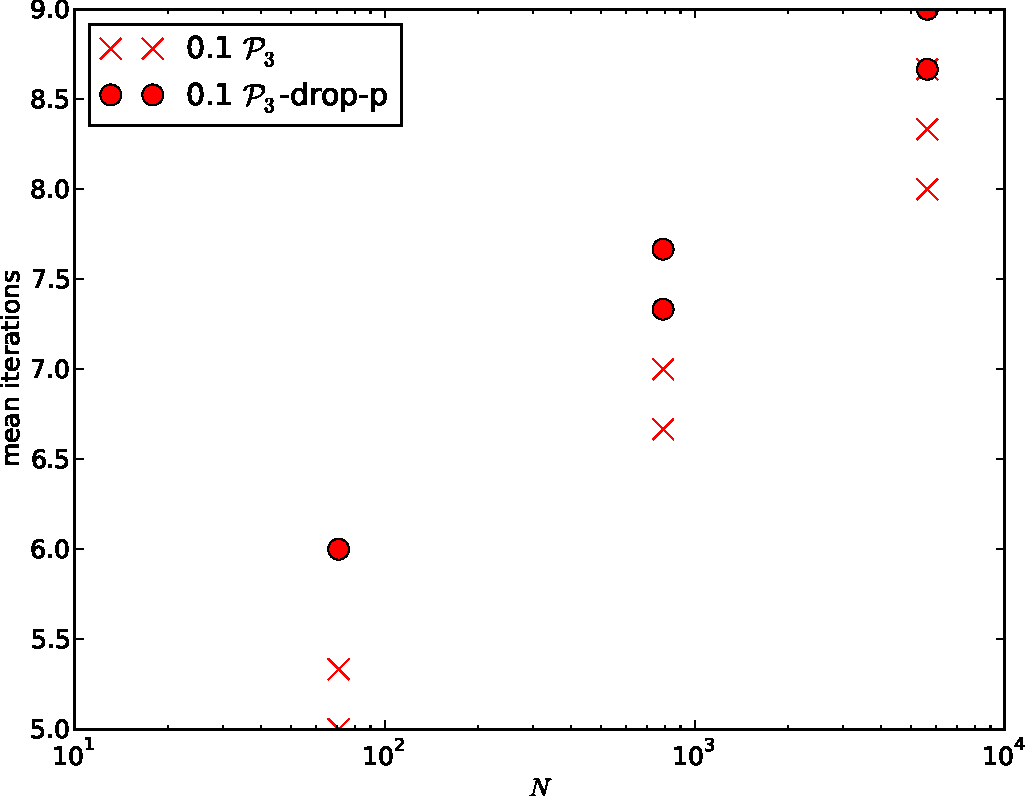
\includegraphics[width=0.8\textwidth]{plots/linear_solvers_p2p3/implicitexact-meanofnsolveritersvsinitialnnode.pdf}
  \caption{GMRES iterations to converge against problem size for the monolithic system using the partially-inexact preconditioners $\parinexact{\precb}$, $\parinexact{\precc}$ with $\dtn=0.1$.
The legend indicates the preconditioner and quadrature scheme used.
}
  \label{fig:its-p23-exact}
\end{figure}

\begin{figure}
  \centering
  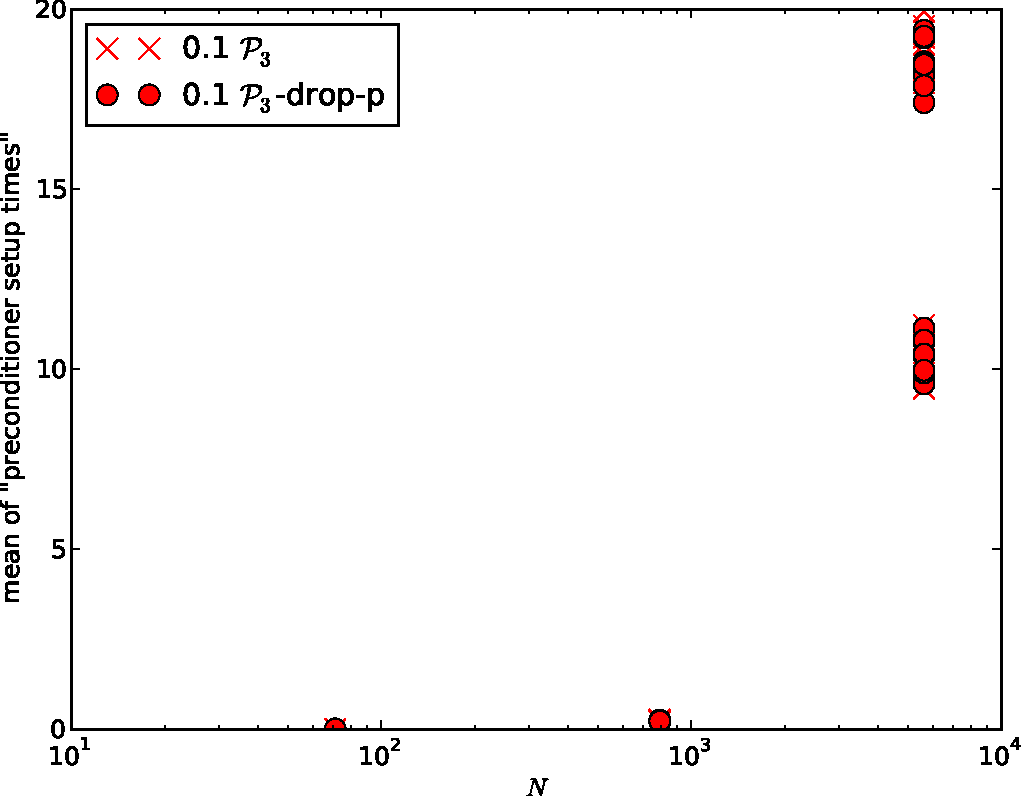
\includegraphics[width=0.8\textwidth]{plots/linear_solvers_p2p3/implicitexact-meanofpreconditionersetuptimesvsinitialnnode.pdf}
  \caption{Time in seconds to set up the partially-inexact preconditioners $\parinexact{\precb}$, $\parinexact{\precc}$ against problem size for the monolithic system with $\dtn=0.1$.
    The legend indicates the preconditioner and quadrature scheme used.
}
  \label{fig:times-p23-exact}
\end{figure}


Finally we show iteration counts for the fully-inexact preconditioners $\inexact{\precb}$ and $\inexact{\precc}$ where the $\Fm$ block is approximated using ILU(1).
We cannot expect $\Nn$-independent results here, since even the simpler case of the solution of the $\Fm$ block alone with GMRES preconditioned by ILU(1) does not display such behaviour.
The iteration counts shown in \cref{fig:its-p23-ilu1}, are as expected: low at first but becoming ineffective for large number of nodes $\Nn$.
In particular, for the largest number of nodes GMRES did not converge within 400 iterations for any of the parameter sets.
Also of note is the much larger variation of the iteration counts with the problem parameters even for the same problem size.
However the preconditioner setup times, as shown in \cref{fig:times-p23-ilu1} are much better than when using the LU decomposition of the $\Fm$ block.

% could try to find/show parameter dependency: some iteration counts are ok!

\begin{figure}
  \centering
  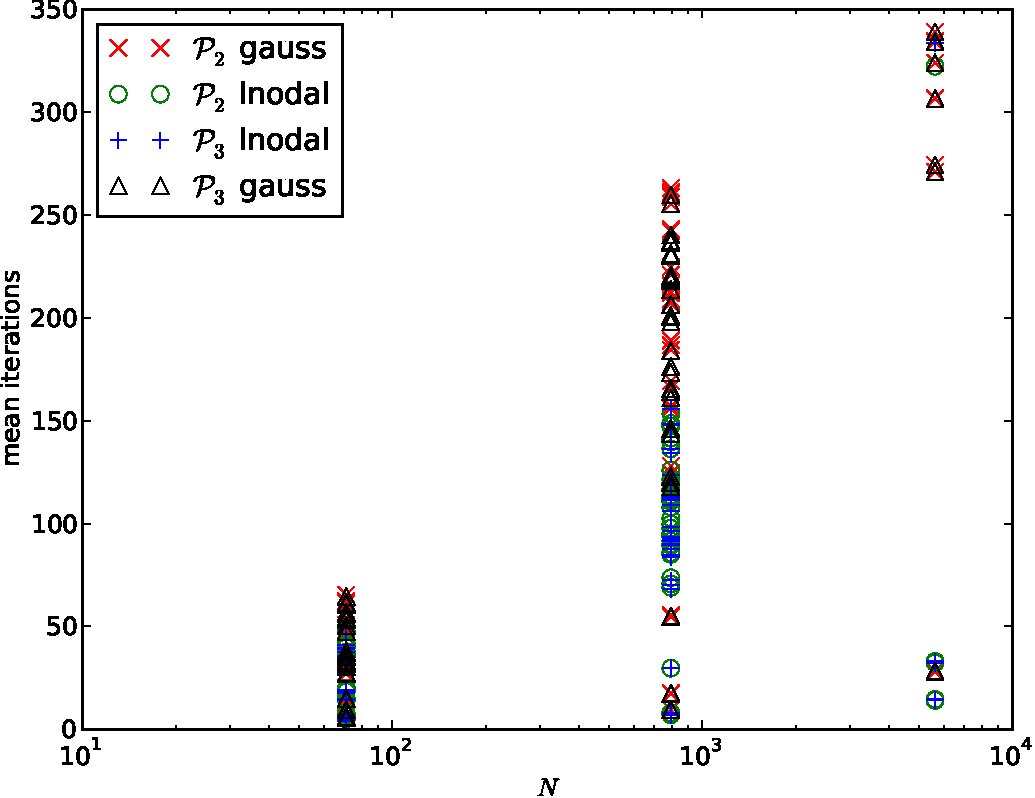
\includegraphics[width=0.8\textwidth]{plots/linear_solvers_p2p3/implicitilu-1-meanofnsolveritersvsinitialnnode.pdf}
  \caption{GMRES iterations to converge against problem size for the monolithic system using the inexact preconditioners $\inexact{\precb}$, $\inexact{\precc}$ with $\dtn=0.1$.
    The legend indicates the preconditioner and quadrature scheme used.
    Some data points are missing for the largest $\Nn$ due to a lack of convergence.
  }
  \label{fig:its-p23-ilu1}
\end{figure}

\begin{figure}
  \centering
  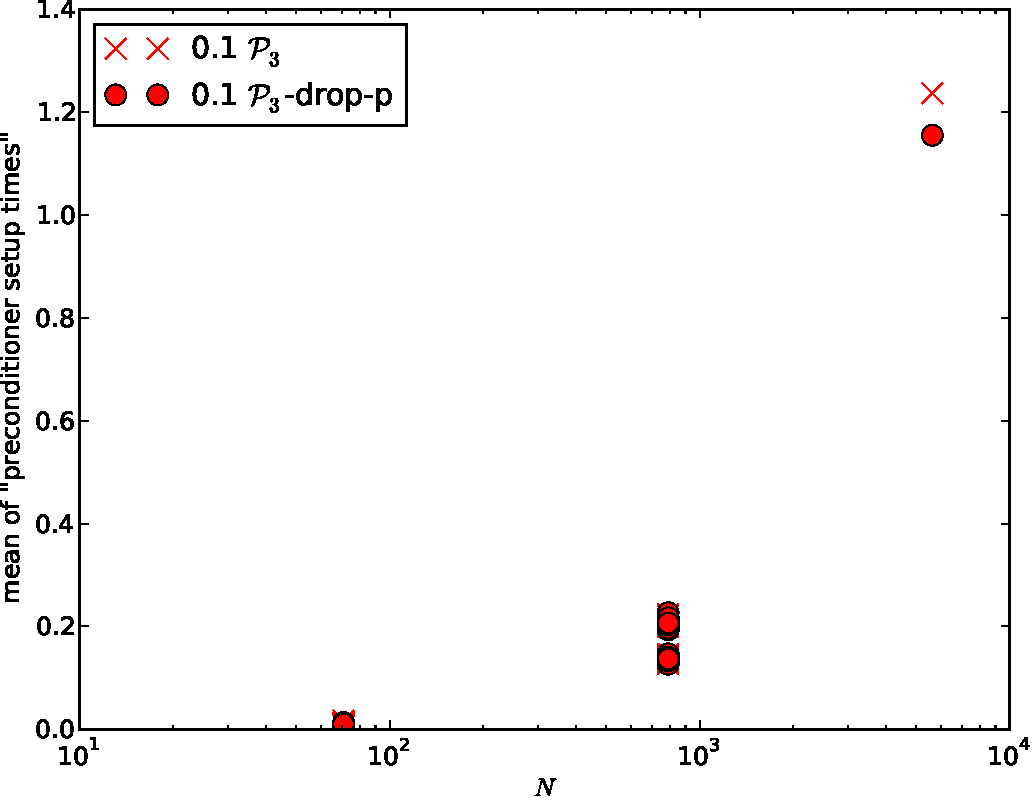
\includegraphics[width=0.8\textwidth]{plots/linear_solvers_p2p3/implicitilu-1-meanofpreconditionersetuptimesvsinitialnnode.pdf}
  \caption{
    Time in seconds to set up the inexact preconditioners $\inexact{\precb}$, $\inexact{\precc}$ against problem size for the monolithic system with $\dtn=0.1$.
    The legend indicates the preconditioner and quadrature scheme used.
    Some data points are missing for the largest $\Nn$ due to a lack of convergence.
  }
  \label{fig:times-p23-ilu1}
\end{figure}

% Effect of HLib? If time do this later


% if I get inner iteration preconditioner working then compare the total solve time for the semi-implicit method (with GMRES and ILU-1 preconditioning) and fully implicit method (with $\precb$, ILU-1 for the $\Fm$ block or maybe using BiCGstab for F?), both using HLib.
% No chance of this now...

\section{Outlook}
\label{sec:furth-optim-opport}

We now compare the \emph{expected} performance of the fully implicit and decoupled approaches with the assumption that a ``sufficiently good'' preconditioner for the $\Fm$ block can be found and discuss further improvements that could be made.

First we examine the relative cost of the assembly of the Jacobian matrices and Newton residuals.
As mentioned above the Jacobian matrices corresponding to linear equations are only dependent  on the geometry and so do not need to be recomputed at each Newton step.
So the Poisson Jacobians and the LLG-Poisson coupling blocks ($\Qm$ and $\Pm$ from \cref{eq:16}) do not need to be recomputed.
This means that for both methods only assembly of the $\Fm$ block is required, and the computation time is identical.

As an aside: the mass matrix blocks on the diagonal of $\Fm$ ($\Mm$ of \cref{eq:llg-jacobian}) are also linear.
Additionally the skew symmetric structure of \cref{eq:llg-jacobian} can be exploited so that the calculation of $\Km_x$ is reused for $-\Km_x$, and similarly for $\Km_y$ and $\Km_z$.
Applying these additional optimisations reduces the Jacobian calculations to the assembly of three $\Nn \times \Nn$ Jacobian blocks and the magnetocrystalline anisotropy block (which will typically be either a single $\Nn \times \Nn$ block or empty, see \cref{sec:llg-jacobian}).

In practice the Newton residual assembly time is extremely small compared to the solve and Jacobian assembly times.
So the computation time difference due to assembling additional $\phim$ and $\phione$ residual components in Newton steps after the first can be ignored.

We now examine the cost per Krylov iteration (or per set of Krylov iterations for the decoupled case).
The monolithic approach has more non-zeros in the Jacobian (the P, Q, G blocks), giving approx $4 \Nn$ extra matrix elements, compared to a base of $11 \Nn$, hence approximately one third as much time again is taken for each Krylov step.
Also our fully coupled method uses GMRES for all blocks rather than GMRES for $\Fm$ and CG for the two Poisson blocks.
Since GMRES requires a more computationally expensive orthogonalisation process than CG this will increase the cost of the monolithic approach as compared to the semi-implicit approach.
This increase could possibly be reduced by using BiCGStab or a restarted GMRES method instead of GMRES.
Finally it is likely that the monolithic method will require more Krylov iterations to converge, but with a good preconditioner for the $\Fm$ block this difference should be fairly small.

Based on all these factors we can estimate that, with an effective preconditioner, the computational time for a monolithic time step should certainly be within a factor of 2 of the time for a decoupled step.


\section{Conclusions and future work}

Monolithic solvers are required for the energy property of IMR, as well as for various other useful properties of implicit time integration schemes.
We have demonstrated that a fully implicit (monolithic) LLG-magnetostatics solver using GMRES with an effective preconditioner can have a computational cost per linear solve close to that of a semi-implicit method.
The partially-inexact preconditioners $\parinexact{\precb}$ and $\parinexact{\precc}$ are able to reduce the iteration count of GMRES extremely effectively and almost independently of the number of nodes, but the set up cost is high for large matrices.
However the fully-inexact equivalents, $\inexact{\precb}$ and  $\inexact{\preca}$, which use ILU(1) to approximate the LLG block are ineffective for more than a few thousand nodes (\ie matrices of size $\sim 10,000$).
Hence cheap, effective and mesh independent approximations for the LLG block, $\Fm$, are still needed for the monolithic block-preconditioned method discussed here to be effective on general large problems.

We have also demonstrated solvers for a decoupled LLG block solve, for medium numbers of nodes it appears that ILU(1) is a good preconditioner for this case.
However, the time integration properties of the semi-implicit scheme using this solve have yet to be seen.


For granular or bit patterned media a domain-decomposition preconditioner exploiting the low/zero exchange coupling between grains/islands could make for a simple but effective domain decomposition preconditioner.
For example, such a preconditioner could be implemented by performing an independent direct solve on the matrix block associated with each grain/island and using this diagonal block solution as the preconditioner.
Since the number of nodes in a single grain/island is likely to be small this would remain effective even for very large numbers of grains/islands.

Reordering of the degrees of freedom, scaling, drop tolerance, fill-in level in the ILU preconditioner could be experimented with further to allow the solution of larger systems or alternative parameters \cite[287]{Saad2000}.
However, ILU preconditioning is unlikely to ever give $\Nn$-independent or parameter-independent results, so it may not be the best path towards more general efficient preconditioners.




%%% Local Variables:
%%% mode: latex
%%% TeX-master: "main"
%%% End:
